\documentclass[runningheads]{llncs}

\usepackage[T1]{fontenc}
% Scalable outline fonts. Without these, microtype's font expansion fails on a
% minimal TeX Live install that ships only bitmap Computer Modern.
\usepackage{lmodern}
\usepackage{graphicx}
\usepackage{booktabs}
\usepackage{amsmath}
\usepackage{amssymb}
\usepackage{amsfonts}
\usepackage{microtype}
\usepackage[hidelinks]{hyperref}

\begin{document}

% The colon in the full title is expressed as an LNCS subtitle, which is the
% class's idiom for it and sets the second part in smaller type.
\title{When Relevance Does Not Transfer}
\subtitle{Consumer-Dependent Retrieval Utility in Sequential Decision Systems}
\titlerunning{When Relevance Does Not Transfer}

\author{Anonymous Author(s)}
\authorrunning{Anonymous}
\institute{Anonymous Institution}

\maketitle

\begin{abstract}
Retrieval is evaluated by relevance, and increasingly by the quality of the
text a language model then generates. A growing class of deployments instead
feeds retrieved evidence to a decision policy, where an error's cost depends on
which action it induces and on how the system evolves afterwards. We build an
executable benchmark for that setting --- an operational report feed, a
retrieval step, a fixed probabilistic interpreter, a fixed controller, and a
simulator that returns realised utility --- and report a negative result. The
value of a ranking is not a property of the ranking. At a matched evidence
budget, every ranking system we test \emph{helps} one downstream consumer and
\emph{harms} another: the retriever~$\times$~consumer interaction changes sign
for all four, and ranking quality orders systems correctly for one consumer
(rank-reversal rate $0.00$) but not the other ($0.33$). The information is
present and extractable --- an oracle relevance selector helps both consumers
--- so the failure is a mismatch between retrieval and its consumer, not an
absence of useful evidence. Supporting diagnostics locate the mismatch:
text-free, shuffled-text and label-only controls show that belief accuracy and
probabilistic sophistication do not imply operational value, and a
perfect-semantic belief reference is not an upper bound on realised return. We
release the benchmark, its frozen artifacts and its controls; every table
regenerates from the stored episodes.
\keywords{Retrieval evaluation \and Downstream utility \and Evidence selection
\and Consumer dependence \and Calibration.}
\end{abstract}

\section{Introduction}
\label{sec:intro}

An operator monitoring a supply network receives a stream of reports. Most
concern other sites; some are stale; a few describe conditions that should
change what they order this period. Choosing which reports to act on is an
information access problem, and its consequences are sequential: an order
placed now arrives several periods later, into a state that earlier decisions
produced.

Standard retrieval evaluation scores such a system by topical relevance, and
downstream-aware evaluation such as eRAG scores it by the quality of the text a
model subsequently generates~\cite{salemi2024erag}. Both treat the value of a
ranking as a property of the ranking. This paper reports that in a
consequential setting it is not.

We ask when retrieved text improves sequential decisions, and make the whole
path executable so the question can be answered rather than argued:

\begin{equation}
\label{eq:path}
q,\,\mathcal{D} \;\longrightarrow\; R_k(q,\mathcal{D}) \;\longrightarrow\;
b(z\mid \cdot) \;\longrightarrow\; \pi(a_t\mid s_t,b) \;\longrightarrow\;
s_{t+1} \;\longrightarrow\; U.
\end{equation}

A retrieval system $R_k$ selects $k$ documents from a candidate pool
$\mathcal{D}$ under a fixed query $q$; a fixed interpreter maps the selected
text to a belief $b$ over operational regimes; a fixed controller maps state and
belief to an action; a simulator returns realised utility $U$. Holding
everything after retrieval constant makes differences in $U$ attributable to
evidence selection. Varying only the interpreter, with retrieval held constant,
isolates the consumer.

\paragraph{The result.}
At $k=3$, every ranking system --- random, BM25, TF--IDF cosine and dense
retrieval --- produces a positive paired effect for a rule-based consumer and a
negative one for a calibrated classifier consumer. The
retriever~$\times$~consumer interaction changes sign in all four cases and
reaches $+89$ reward units. Ranking quality orders systems exactly as realised
utility does for the first consumer and disagrees on a third of pairs for the
second. The evidence itself is not the problem: an oracle relevance selector
improves \emph{both} consumers, by $+60.6$ and $+69.0$ respectively. What fails
is the match between what practical rankers retrieve and what a particular
consumer does with it.

\paragraph{Contributions.}
(i) An executable benchmark that scores evidence selection by the sequential
decision utility it induces, with retrieval quality reported on the same
episodes (Section~\ref{sec:retrieval}).
(ii) A measured negative result --- consumer-dependent retrieval utility ---
reported as an interaction, a rank-reversal rate, episode-level correlations and
a harmful-retrieval rate rather than a single headline number.
(iii) Diagnostics that locate the mismatch: text-free, shuffled-text and
label-only controls showing that belief accuracy and probability quality do not
imply operational value (Section~\ref{sec:diagnosis}).
(iv) A reproducible artifact with the estimand, weighting and uncertainty
declared, in which every table in this paper regenerates from the stored
episodes.

\paragraph{Scope.} The report feed and environments are synthetic. We introduce
no retrieval model and claim no interpreter or controller is preferable in
general. The claim is about \emph{evaluation}: a retrieval system that feeds a
decision policy cannot be scored independently of that policy, and the controls
needed to support such a claim are stronger than those usually reported.

\section{Related work}
\label{sec:related}

\paragraph{Downstream-aware retrieval evaluation.}
eRAG evaluates retrieval by the downstream performance of the language model
that consumes it, showing that upstream relevance can be a poor proxy for
end-task utility~\cite{salemi2024erag}. CUE-R estimates per-evidence utility by
intervention and includes no-retrieval controls; GroGU argues grounding utility
is consumer-specific. Both are recent preprints and we treat them as
such~\cite{cuer2026,grogu2026}. Our downstream consumer is a control policy in a
stochastic environment rather than a generator, so the estimated quantity is a
trajectory's realised return, not text quality, and the error asymmetry comes
from the environment's cost structure rather than a judge. Where GroGU argues
for consumer specificity, we measure it end to end and find it strong enough to
reverse the sign of a ranking's value. That relevance is situational and
task-dependent long predates this work~\cite{borlund2003concept}; the
contribution here is an instrument for one consequential task, not the
observation that consequences matter.

\paragraph{Decision-focused prediction and calibration.}
Predict-then-optimize and decision-focused learning train or evaluate
predictions through a downstream
objective~\cite{donti2017task,elmachtoub2022smart,mandi2022rank}; value-aware
model learning makes the analogous point for learned
dynamics~\cite{farahmand2017value,lambert2020objective}, decision calibration
formalises dependence on a decision-maker~\cite{zhao2021decision}, and
value-of-information theory gives the classical account of when information
changes a decision~\cite{howard1966information}. Probability quality is
standardly assessed with proper scores and calibration
diagnostics~\cite{guo2017calibration,degroot1983comparison,niculescu2005predicting}.
We do not learn through the objective: we hold the pipeline fixed and vary what
is supplied to it, which makes this an evaluation rather than a training method.

\paragraph{Environment and baselines.}
The multi-echelon simulator derives from an inventory benchmark lineage in
operations research~\cite{hubbs2020orgym} and is used at a pinned published
version~\cite{gyminvmgmt}. Retrieval baselines are Okapi
BM25~\cite{robertson1994okapi} and cosine similarity over sentence
embeddings~\cite{reimers2019sentencebert}, scored with
nDCG~\cite{jarvelin2002cumulated}.

\section{Framework}
\label{sec:framework}

\subsection{Objects and estimand}

Let $z$ be a latent operational regime, $\mathcal{D}$ a candidate pool of
reports and $q$ a fixed query expressing a standing information need. A
retrieval system returns an ordered list; its top $k$ documents are the
evidence. A fixed interpreter maps their concatenation to a belief $b(z)$, and a
fixed controller maps state and belief to an action.

Write $G_i(m)$ for the \emph{realised} return of episode $i$ under information
source $m$, $G_i(m)=\sum_{t=0}^{T-1} r(s^{(i)}_t,a^{(i)}_t,z^{(i)})$,
undiscounted: the horizon is finite and fixed at $T=40$, and any discounting
inside the environment is part of $r$. We keep realised returns distinct from
their expectation, which we estimate by the weighted benchmark return
\begin{equation}
\label{eq:jw}
J_w(m) \;=\; \sum_{r} w_r \,
\operatorname*{mean}_{f \in \mathcal{F}_r} \;
\operatorname*{mean}_{v \in \mathcal{V}_{r,f}} \;
\operatorname*{mean}_{i \in \mathcal{S}} \; G_i(m; r, f, v),
\end{equation}
averaging seeds within a template variant $v$, variants within an ambiguity
family $f$, families within a regime $r$, and combining regimes with declared
weights $w_r$. The \emph{balanced} estimand uses uniform $w_r$ and is primary; a
deployment-prior estimand is secondary. Group sizes are unequal, so
\eqref{eq:jw} is not an equal-row mean over episodes, and the difference is
numerically material.

Effects are reported as paired differences $\Delta J$ against a declared
reference: for retrieval, a control that retrieves nothing; for interpreters,
the uninformed prior. Where a normalised diagnostic is used, its numerator and
denominator carry identical weights. We report it sparingly: the
\emph{perfect-semantic reference} --- a correct belief passed through the fixed
controller --- is demonstrably not an upper bound on realised return
(Section~\ref{sec:diagnosis}), so normalising by it does not yield a recovered
fraction of anything.

\subsection{Uncertainty}
\label{sec:uncertainty}

The design crosses worlds (seeds) with language (templates): every template
within a regime is evaluated on the same seeds, so seeds are not independent
draws nested under templates. We resample the two axes independently --- one
\emph{shared} seed sample per regime, reused by every family and variant, plus
families and variants with replacement. Intervals are percentile intervals from
$B$ replicates; $p$-values are centred bootstrap test inversions,
$(1+\#\{|b^\ast-\hat\theta|\ge|\hat\theta|\})/(B+1)$, bounded below by $1/(B+1)$
and never reported as exactly zero. With three designed ambiguity families per
regime the family axis is small, so intervals are conditional on the fixed
template set and generalisation to new language remains open.

\section{Experiment R: consumer-dependent retrieval utility}
\label{sec:retrieval}

\subsection{Setup}

Each episode is a (seed, regime) pair. The candidate pool holds four kinds of
document, all in the same operational register: \emph{relevant}, a current
report about the operator's own node; \emph{wrong entity}, a current report
about a different node, drawn across all regimes so that some of these errors
actively mislead and some are accidentally correct; \emph{stale}, the operator's
node but an event already marked resolved; and \emph{off-topic}, routine
corporate traffic attributed to the operator's node so that it cannot be
filtered on entity alone.

Relevance is determined by the query --- entity and recency --- and never by
regime; identifying the regime is the interpreter's job. That separation is what
makes the retrieval task solvable and the dissociation measurable.

Systems: random (floor), BM25, TF--IDF cosine, dense sentence-embedding cosine,
and an oracle relevance selector; a no-retrieval control supplies the paired
reference. Evidence budgets $k\in\{1,3,5\}$ are matched across systems. The two
consumers are a rule-based extractor and a calibrated TF--IDF classifier; the
controller is a receding-horizon optimiser and is identical throughout.

\begin{table}[t]
\caption{Experiment~R. Retrieval quality and downstream decision utility on the
same episodes, at a matched evidence budget $k=3$, with the calibrated TF--IDF
interpreter and the receding-horizon controller held fixed. $\Delta J$ is the
paired effect against the no-retrieval control; intervals are crossed bootstrap
percentile intervals with shared seed draws.}
\label{tab:retrieval}
\centering\small
\begin{tabular}{lrrrrr}
\toprule
System & nDCG@3 & R@3 & MRR & $J_w$ & $\Delta J$ (95\% CI) \\
\midrule
No retrieval & 0.000 & 0.000 & 0.000 & 1657.2 & +0.0~[+0.0, +0.0] \\
Random & 0.090 & 0.117 & 0.218 & 1607.4 & -49.8~[-78.0, -18.8] \\
BM25 & 0.274 & 0.294 & 0.444 & 1583.0 & -74.3~[-98.9, -47.9] \\
TF--IDF cosine & 0.336 & 0.356 & 0.517 & 1596.1 & -61.1~[-88.4, -31.6] \\
Dense (MiniLM) & 0.617 & 0.672 & 0.727 & 1655.7 & -1.5~[-31.1, +29.2] \\
Oracle selector & 1.000 & 1.000 & 1.000 & 1726.2 & +69.0~[+40.2, +96.1] \\
\bottomrule
\end{tabular}
\end{table}


\subsection{The retrieval task is solvable, and the evidence is there}

Ranking quality orders the systems random $<$ BM25 $<$ TF--IDF cosine $<$ dense
$<$ oracle, with a wide spread in nDCG@3 (Table~\ref{tab:retrieval}), and the
rate at which retrieved documents actively mislead falls monotonically along the
same ordering, from $0.44$ for random to $0.22$ for the oracle selector. The
oracle relevance selector improves \emph{both} consumers, by $+60.6$
$[+48,+73]$ and $+69.0$ $[+40,+96]$. Selecting the right evidence from this pool
is therefore both possible and worth doing, for either consumer.

\subsection{But its value is not a property of the ranking}

\begin{figure}[t]
\centering
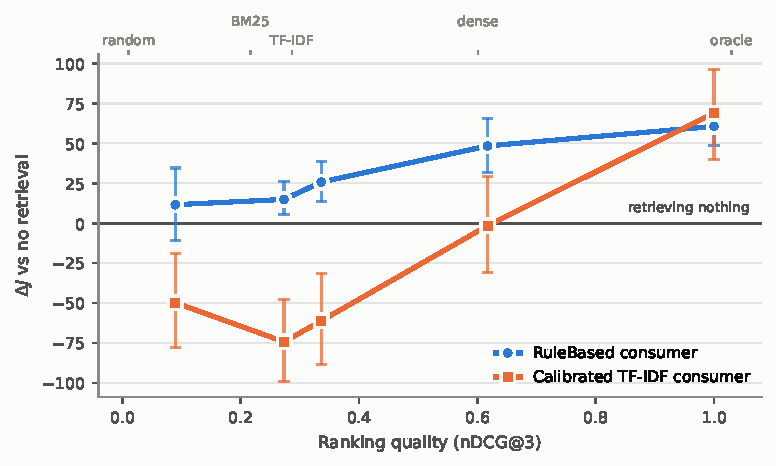
\includegraphics[width=0.86\textwidth]{figures/interaction}
\caption{The same rankings, two consumers, one zero line. The horizontal axis is
a property of the retrieval alone; the vertical axis is what that retrieval
turned out to be worth, as a paired effect against retrieving nothing (bars are
95\% crossed bootstrap intervals). Across the whole practical range the two
consumers sit on opposite sides of zero, converging only at the oracle
selector. A relevance-only evaluation observes the horizontal axis and cannot
distinguish the two situations.}
\label{fig:interaction}
\end{figure}

\begin{table}[t]
\caption{Experiment~R. How much of a ranking's value belongs to the ranking?
Left: the retriever~$\times$~consumer interaction at $k=3$ --- the difference
between the two consumers' paired effects for the same ranking. Every
interaction changes sign, so no single number describes what a ranking is
worth. Right: within each consumer, how often ranking quality orders two
systems the way realised utility does, and how strongly the two correlate
across episodes.}
\label{tab:consumerdep}
\centering\small
\begin{tabular}{@{}l rrr c@{}}
\toprule
System & RuleBased $\Delta J$ & Calibrated $\Delta J$ & Interaction & Sign flip \\
\midrule
Random & +11.6 & -49.8 & +61.4 & \checkmark \\
BM25 & +14.9 & -74.3 & +89.2 & \checkmark \\
TF--IDF cosine & +25.8 & -61.1 & +86.9 & \checkmark \\
Dense (MiniLM) & +48.4 & -1.5 & +49.9 & \checkmark \\
\bottomrule
\end{tabular}

\vspace{0.6em}

\centering\small
\begin{tabular}{@{}l rrrr@{}}
\toprule
Consumer & Reversal rate & Kendall $\tau_b$ & Pearson $r$ & Spearman $\rho$ \\
\midrule
RuleBased & 0.00 (0/6) & +1.00 & +0.372 & +0.392 \\
Calibrated TF--IDF & 0.33 (2/6) & +0.33 & +0.382 & +0.367 \\
\bottomrule
\end{tabular}

\vspace{0.6em}

\centering\small
\begin{tabular}{@{}l rrr@{}}
\toprule
Dense retrieval at budget $k$ & $k=1$ & $k=3$ & $k=5$ \\
\midrule
nDCG@$k$ & 0.556 & 0.617 & 0.691 \\
RuleBased $\Delta J$ & +21.3 & +48.4 & +46.0 \\
Calibrated TF--IDF $\Delta J$ & -69.3 & -1.5 & -18.9 \\
\bottomrule
\end{tabular}
\end{table}


Every practical ranking system helps the rule-based consumer and harms the
calibrated one (Figure~\ref{fig:interaction}). Dense retrieval is $+48.4$ $[+32,+65]$ for the first and $-1.5$
$[-31,+29]$ for the second; BM25 is $+14.9$ $[+5,+26]$ and $-74.3$ $[-99,-48]$.
The retriever~$\times$~consumer interaction changes sign for all four systems
and ranges from $+49.9$ to $+89.2$ reward units
(Table~\ref{tab:consumerdep}). There is no single number that describes what
BM25 is worth here.

Ranking quality inherits that ambiguity. For the rule-based consumer the nDCG
ordering and the utility ordering agree on every pair (rank-reversal rate
$0.00$, $\tau_b=+1.00$); for the calibrated consumer they disagree on a third of
pairs ($0.33$, $\tau_b=+0.33$). An evaluator who selected a retriever on nDCG
would be right every time for one consumer and wrong a third of the time for the
other, with no upstream signal distinguishing the two situations.

\subsection{The gradient is shared; the level is not}

The episode-level correlation between ranking quality and realised reward is
almost identical for the two consumers ($r=+0.372$ and $+0.382$;
$\rho=+0.392$ and $+0.367$), computed within episodes so that episode
difficulty cannot dominate. This is worth stating precisely, because it narrows
the claim. \emph{Within} a consumer, better evidence does produce better
decisions, and to a similar degree for both. What differs is the level: the
calibrated consumer is worse than retrieving nothing across the whole practical
range, and only reaches parity once retrieval is near-oracle. Consumer
dependence here is an offset, not a reversed gradient --- which is precisely why
a relevance-only evaluation cannot detect it.

\subsection{More evidence is not better}

The last panel of Table~\ref{tab:consumerdep} follows the strongest ranker
across budgets. Moving from $k=3$ to $k=5$ raises dense retrieval's nDCG
($0.617 \to 0.691$) while lowering its effect on the calibrated consumer
($-1.5 \to -18.9$) and leaving the rule-based consumer flat
($+48.4 \to +46.0$). The extra documents are mostly non-relevant, and neither
consumer has a mechanism for discounting them --- but only one of them pays for
that.

\section{Locating the mismatch}
\label{sec:diagnosis}

Why does one consumer convert better evidence into better decisions while the
other does not? We hold retrieval aside and vary the belief directly, in two
transfer environments: a held-out multi-echelon demand-surge setting
(Experiment~M) and a supply-side capacity drop (Experiment~S). Alongside the
interpreters we run constant-belief endpoints, a no-text operating point tuned
only on development seeds, a shuffled-text ablation in which the interpreter
reads a real warning belonging to a different template, and a label-only
ablation that discards the interpreter's probabilities.

\begin{table}[t]
\caption{Experiment~M (held-out multi-echelon transfer, demand surge). Rows are grouped as text-free controls, text interpreters, degraded-text controls, and the oracle-belief reference. $J_w$ is the balanced weighted return; $\Delta J$ is the paired effect against NoInfo. A dev-tuned constant belief that reads no text is the row every interpreter must beat.}
\label{tab:expM}
\centering\small
\begin{tabular}{lrrlrr}
\toprule
Information source & $J_w$ & $\Delta J$ & 95\% CI & $p$ & SIVR \\
\midrule
NoInfo (prior) & 467.7 & +0.0 & [+0.0, +0.0] & 1.000 & 0.000 \\
Constant $p_{\mathrm{event}}=0$ & 381.2 & -86.5 & [-93.5, -80.1] & $<$0.0002 & -1.027 \\
Constant $p_{\mathrm{event}}=0.5$ & 501.1 & +33.3 & [+32.2, +34.8] & $<$0.0002 & 0.396 \\
Constant $p_{\mathrm{event}}=1$ & 560.4 & +92.7 & [+89.5, +95.8] & $<$0.0002 & 1.100 \\
\textbf{No-text (dev-tuned)} & 560.4 & +92.7 & [+89.5, +95.8] & $<$0.0002 & 1.100 \\
\midrule
RuleBased & 568.7 & +101.0 & [+94.7, +106.0] & $<$0.0002 & 1.198 \\
TF--IDF (single) & 516.2 & +48.5 & [+36.5, +58.4] & $<$0.0002 & 0.575 \\
TF--IDF (calib., isotonic) & 530.2 & +62.5 & [+4.7, +95.8] & 0.017 & 0.742 \\
GPT-4o & 534.9 & +67.1 & [+29.7, +87.2] & 0.002 & 0.797 \\
\midrule
TF--IDF cal.\ (label only) & 523.5 & +55.8 & [-23.5, +89.4] & 0.066 & 0.662 \\
TF--IDF cal.\ (shuffled) & 451.1 & -16.6 & [-67.3, +51.8] & 0.578 & -0.198 \\
Oracle belief & 552.0 & +84.3 & [+76.8, +91.1] & $<$0.0002 & 1.000 \\
\bottomrule
\end{tabular}
\end{table}

\begin{table}[t]
\caption{Experiment~S (supply-side capacity-drop transfer). Same protocol, a structurally different event mechanism.}
\label{tab:expS}
\centering\small
\begin{tabular}{lrrlrr}
\toprule
Information source & $J_w$ & $\Delta J$ & 95\% CI & $p$ & SIVR \\
\midrule
NoInfo (prior) & 1333.6 & +0.0 & [+0.0, +0.0] & 1.000 & 0.000 \\
Constant $p_{\mathrm{event}}=0$ & 1166.7 & -166.9 & [-166.9, -166.9] & $<$0.0002 & -1.481 \\
Constant $p_{\mathrm{event}}=0.5$ & 1333.6 & +0.0 & [+0.0, +0.0] & 1.000 & 0.000 \\
Constant $p_{\mathrm{event}}=1$ & 1725.1 & +391.5 & [+386.6, +395.8] & $<$0.0002 & 3.473 \\
\textbf{No-text (dev-tuned)} & 1725.1 & +391.5 & [+386.6, +395.8] & $<$0.0002 & 3.473 \\
\midrule
RuleBased & 1447.0 & +113.4 & [+39.1, +183.1] & 0.003 & 1.006 \\
TF--IDF (single) & 1362.8 & +29.2 & [-3.9, +68.5] & 0.136 & 0.259 \\
TF--IDF (calib., isotonic) & 1372.9 & +39.3 & [-73.0, +130.7] & 0.467 & 0.349 \\
GPT-4o & 1372.6 & +38.9 & [-39.0, +85.2] & 0.271 & 0.345 \\
\midrule
TF--IDF cal.\ (label only) & 1392.0 & +58.4 & [-72.8, +114.9] & 0.112 & 0.518 \\
TF--IDF cal.\ (shuffled) & 1415.2 & +81.6 & [-66.8, +257.9] & 0.327 & 0.724 \\
Oracle belief & 1446.3 & +112.7 & [+109.2, +115.6] & $<$0.0002 & 1.000 \\
\bottomrule
\end{tabular}
\end{table}


\paragraph{A text-free control is a demanding baseline.}
In Experiment~M the development-tuned no-text control returns $560.4$, above
single TF--IDF ($516.2$), calibrated TF--IDF ($530.2$) and GPT-4o ($534.9$);
only the rule-based interpreter ($568.7$) exceeds it. In Experiment~S it returns
$1725.1$ against $1447.0$ for the best interpreter. Reward increases
monotonically in the assumed event probability, so the controller is
systematically under-positioned under the benchmark prior and any belief that
raises the order-up-to level captures part of that gap without reading anything.
This is the same failure mode that makes the calibrated consumer fragile in
Experiment~R: its value depends on where its belief mass sits relative to the
controller's operating point, not only on whether the belief is right.

\paragraph{Belief accuracy does not imply operational value.}
In Experiment~S the shuffled-text control returns $1415.2$, \emph{above} the
genuine interpreter's $1372.9$, at roughly half the belief accuracy. Whatever
that interpreter gains there comes from the shape of its belief distribution,
not from identifying the regime. In Experiment~M shuffling does destroy the
effect ($530.2 \to 451.1$, below the uninformed prior), so reading the correct
text is doing real work in one environment and not the other.

\paragraph{Probabilistic sophistication does not either.}
Collapsing the calibrated interpreter to its hard label costs little in
Experiment~M ($530.2 \to 523.5$) and helps in Experiment~S
($1372.9 \to 1392.0$). In the controlled benchmark the label-only ablation of
the raw classifier reaches a normalised value of $0.773$ against $0.245$ for its
own probabilities, with a better Brier score ($0.222$ versus $0.552$) and a much
worse log-loss ($2.558$ versus $0.932$): the two proper scores disagree about
it, and neither predicts its operational advantage.

\paragraph{Calibration is not an isolated intervention.}
\texttt{CalibratedClassifierCV} fits one classifier per fold and averages them,
so a raw-versus-calibrated contrast mixes a calibration map with an ensembling
change. Adding the missing arm --- the same fold ensemble with no calibration
map --- separates them: ensembling alone \emph{lowers} normalised value
($0.245 \to 0.154$) and the calibration map then recovers past it
($\to 0.338$). The direction survives; the naive difference is not attributable
to calibration.

\paragraph{The perfect-semantic reference is not an upper bound.}
A correct belief passed through the fixed controller is beaten by a constant
belief that reads nothing, in both transfer environments
(Table~\ref{tab:transfers}). We therefore call it a reference rather than an
oracle, and avoid normalising by it where a raw paired effect will do.

\section{Boundaries and limitations}
\label{sec:limitations}

\begin{table}[t]
\caption{Experiment~B. \emph{Every} one-factor-at-a-time variant, including
the adverse ones. Values are the balanced weighted return $J_w$; OIV is the
oracle information value. $\dagger$ marks a variant whose OIV is not positive:
there the oracle-belief reference itself underperforms the uninformed prior, so
a normalised ratio cannot be read as recovery of information value and the
finding is about controller--environment mismatch, not semantic sensing.}
\label{tab:boundary}
\centering\small\setlength{\tabcolsep}{4pt}
\begin{tabular}{lrrrrrrr}
\toprule
Variant & NoInfo & No-text & Rule & TF--IDF & GPT-4o & Oracle & OIV \\
\midrule
baseline & 1324 & 1713 & 1436 & 1362 & 1362 & 1435 & +112 \\
high\_noise & 1313 & 1674 & 1417 & 1344 & 1346 & 1411 & +97 \\
long\_lead$^{\dagger}$ & -876 & -967 & -902 & -869 & -863 & -878 & -3 \\
lost\_sales$^{\dagger}$ & 1512 & 1439 & 1489 & 1503 & 1507 & 1490 & -22 \\
low\_noise & 1334 & 1732 & 1449 & 1375 & 1372 & 1450 & +116 \\
short\_lead$^{\dagger}$ & 2398 & 2486 & 2411 & 2248 & 2213 & 2214 & -183 \\
\bottomrule
\end{tabular}
\end{table}


Perturbing one environment factor at a time shows how conditional these
quantities are. In three of six variants the perfect-semantic reference itself
underperforms the uninformed prior, so no normalised information-value statement
is meaningful there and we mark rather than report a ratio. Under short lead
times the calibrated interpreter returns $2248$ and GPT-4o $2213$ against the
uninformed prior's $2398$: halving the lead time leaves too little time to act,
so a belief that shifts stock upward mostly buys holding cost.

The report feed and environments are synthetic, single-SKU and finite-regime.
Experiment~R's pools are generated rather than authored, so it carries no
language-axis variance; its query is fixed and relevance is defined by
construction rather than by assessors, which makes the oracle selector a ceiling
for \emph{these} judgments rather than for downstream utility in general. Two
consumers do not establish the shape of consumer dependence, only that it is
large enough to reverse a sign. The dense retriever is one general-purpose
sentence encoder with frozen embeddings, not a trained dense retrieval system.
The controller is fixed and not jointly optimised with the interpreter. Cached
LLM outputs cover a small set of models with reconstructed rather than certified
provenance. Evidence is consumed by concatenation; belief-level pooling over
separately interpreted documents is a natural variant we do not evaluate.

\section{Conclusion}
\label{sec:conclusion}

In a setting where retrieved text drives a decision policy, the value of a
ranking is not a property of the ranking. Every retrieval system we tested helps
one consumer and harms another, the interaction changes sign in every case, and
relevance-based evaluation is a reliable guide for one consumer and unreliable
for the other with nothing upstream to distinguish them. The evidence is
extractable --- an oracle selector helps both --- so this is a mismatch problem,
not a scarcity problem. For evaluation practice the implication is narrow and
concrete: a retrieval component intended for a decision-making consumer should
be scored against that consumer, with a no-retrieval control and a matched
budget, and a reported improvement in relevance should not be assumed to
survive the handoff.

\appendix
\section{Design, accounting and reproduction}
\label{app:design}

\begin{table}[!ht]
\caption{Experiment accounting, generated from the saved episode files rather
than from design intent. `Episodes' counts rows across all information sources;
the number of \emph{paired worlds} is seeds $\times$ templates.}
\label{tab:accounting}
\centering\small
\begin{tabular}{lrrrr}
\toprule
Experiment & Seeds & Templates & Sources & Episodes \\
\midrule
R (retrieval) & 30 & 1 & 6 & 3,240 \\
C (controlled) & 20 & 36 & 12 & 8,640 \\
M (multi-echelon) & 30 & 24 & 12 & 8,640 \\
S (supply-side) & 30 & 16 & 12 & 5,760 \\
\bottomrule
\end{tabular}
\end{table}

\paragraph{No-text operating point (Experiment~M).}
Selected $p_{\mathrm{event}}=1.0$ on development seeds 3200--3229, which are disjoint from every confirmation seed range. Selection used the balanced estimand. The arm is tuned, but never on its own evaluation data.

\paragraph{No-text operating point (Experiment~S).}
Selected $p_{\mathrm{event}}=1.0$ on development seeds 4200--4229, which are disjoint from every confirmation seed range. Selection used the balanced estimand. The arm is tuned, but never on its own evaluation data.


\paragraph{Environment, costs and timing.}
Single-item lost-sales inventory over a finite horizon of $T=40$ periods:
revenue $10$ per unit sold, ordering cost $5$ fixed plus $2$ per unit, holding
cost $1$ per unit of ending inventory, stockout penalty $8$ per unit of unmet
demand, initial on-hand $30$, Poisson demand with base mean $8$. Three regimes:
\textsc{normal}; \textsc{supplier delay}, raising the lead time during the event
window; and \textsc{demand surge}, multiplying the demand rate. The supply-side
transfer instead reduces a factory's capacity in a multi-echelon network. Within
a period the order is: receive arrivals, realise demand, fulfil from on-hand,
place an order. An order placed in period $t$ under lead time $L$ arrives at the
start of period $t+L$; orders already in transit keep their arrival period, so a
lead-time change applies only to orders placed from that period onward. The
simulator and every planner share one implementation of this schedule.

\paragraph{Information release.}
Warning text is published at period $12$; the event window begins at period
$20$. Before publication no interpreter has read anything and every controller
plans under the benchmark prior. From publication the interpreted belief
replaces the prior while on-hand stock and the in-transit pipeline carry over.

\paragraph{Belief to action.}
The controlled experiments solve a receding-horizon linear program each period
and execute only its first order, with belief-weighted expected lead time and
demand per future period. The multi-echelon experiments use a belief-adaptive
base-stock policy with effective rate $\mathbb{E}_b[\mu]$ and order-up-to target
$\mathbb{E}_b[\mu]\bar{L} + 1.65\sqrt{\bar{L}\,\mathbb{E}_b[\mu]}$. The
controller is identical across information sources within an experiment.

\paragraph{Interpreters, information and retrieval.}
No non-oracle interpreter receives the regime, future demand, future state or
environment internals. The TF--IDF classifiers are fitted only on training
templates and evaluated on disjoint held-out ones. LLM beliefs are replayed from
frozen canonical responses, with model labels reconstructed by re-deriving each
cache key from every known (model, text) pair and unmatched entries labelled
\texttt{unknown}. BM25 uses the Okapi form with $k_1=1.5$, $b=0.75$ and idf
floored at zero; dense retrieval is cosine similarity over frozen
\texttt{all-MiniLM-L6-v2} embeddings, shipped so the published numbers reproduce
without model weights. Ties break by document id.

\paragraph{Reproduction.}
The release reconstructs its own offline inputs: cached semantic responses come
from a tracked, checksum-verified manifest, and classifier checkpoints are
retrained from tracked templates with fixed seeds; neither step needs
credentials or network access. The multi-echelon simulator is a pinned published
package~\cite{gyminvmgmt}, and every stored episode replays through it to its
recorded reward exactly. A verification entry point regenerates every table in
this paper from the stored episodes and fails if any differs. This paper shows
that a decision-support component can look better on upstream metrics while
being worse to act on, so deployment needs human oversight and conservative
fallbacks; a synthetic study does not establish deployment safety.

% Marker for an exact content-page count: ECIR allows 12 content pages
% including appendices, with unlimited reference pages. Read this label's page
% from main.aux; counting pages shipped before LaTeX reads main.bbl is wrong,
% because pages are shipped lazily.
\label{endofcontent}

\bibliographystyle{splncs04}
\bibliography{references}

\end{document}
